\documentclass[titlepage]{article}

\usepackage{
	geometry,
	multicol,
	pdfpages
}

\geometry{
	letterpaper,
	margin=1in
}

\setlength{\columnsep}{0.25in}

\title{
	\textbf{
		CSCE 221 --- 200 \\
		Programming Assignment 4 \\
		Final Report
	}
}

\author{
	James Corder Guy \\
	Nathan Powell
}

\date{
	\today
}

\begin{document}
	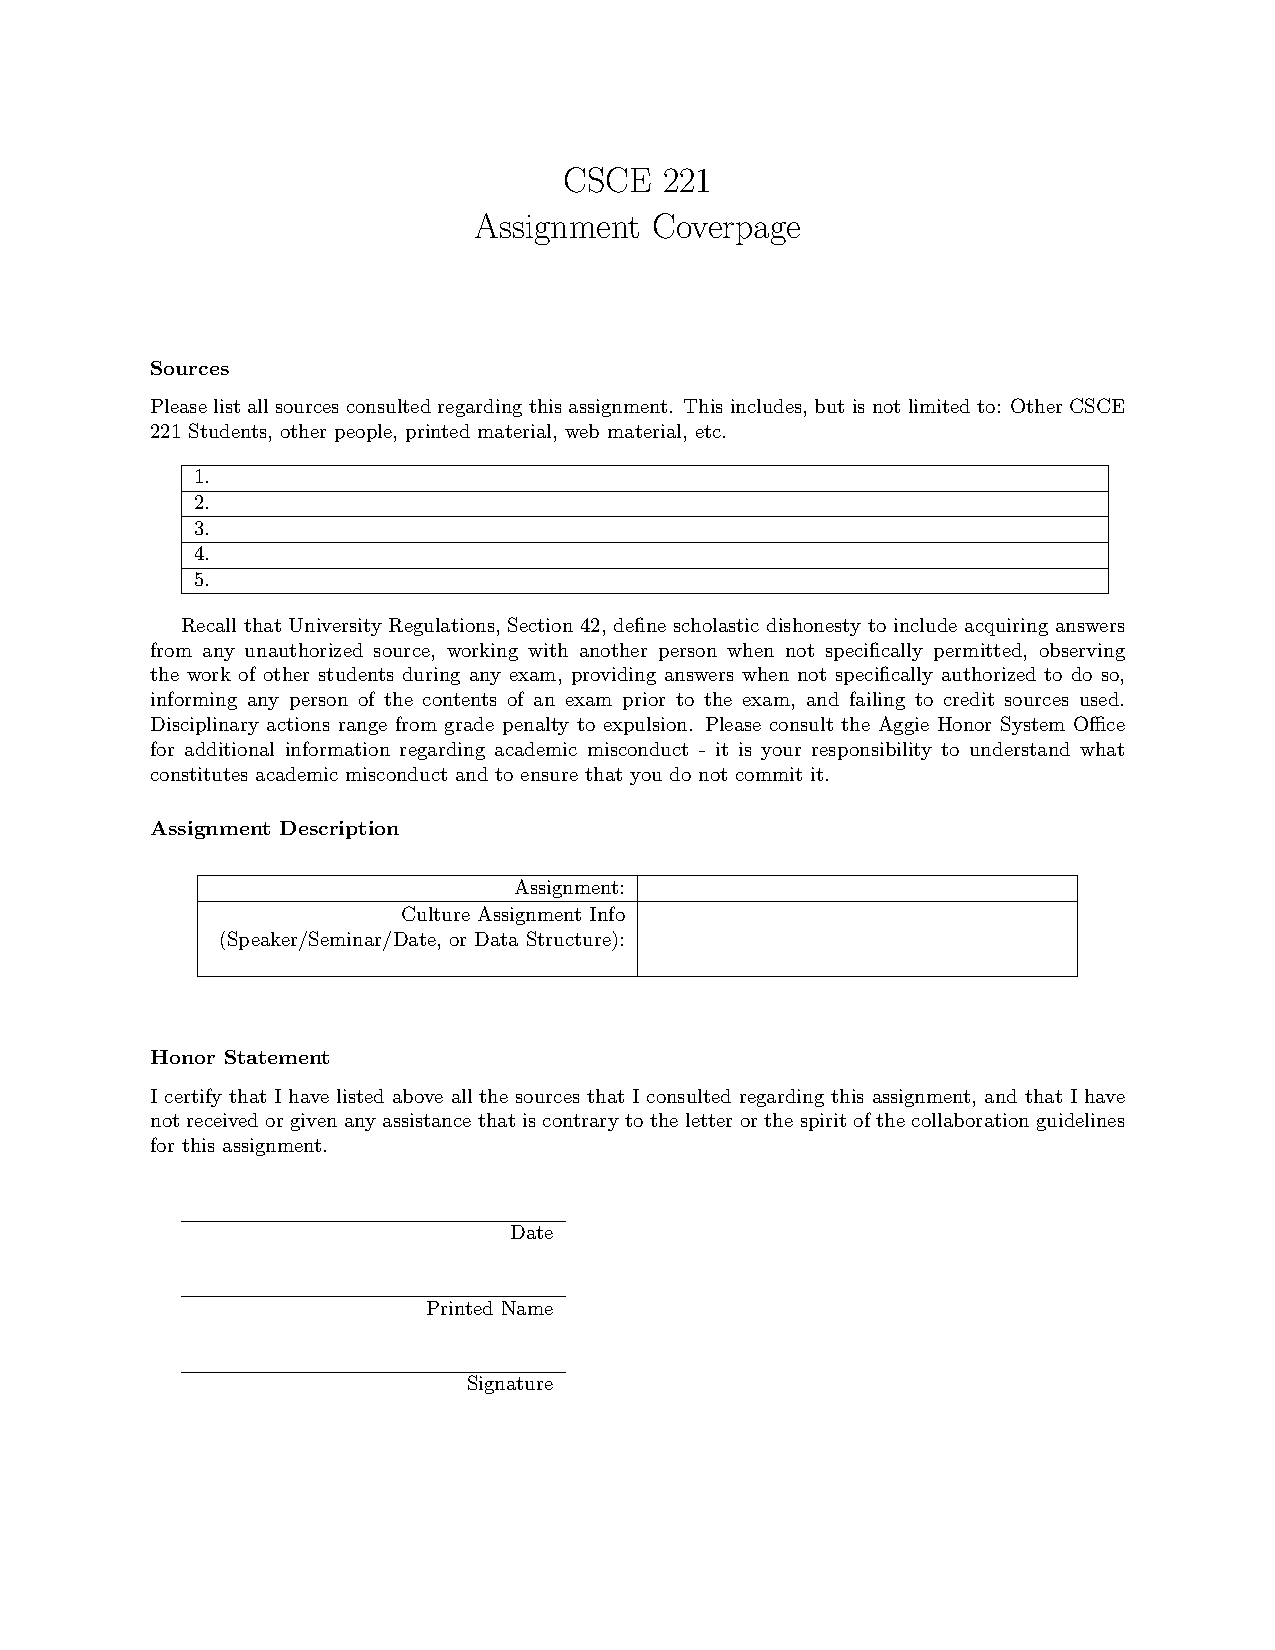
\includepdf[pages={-}]{./coverpage.pdf}
	\maketitle
	\begin{multicols}{2}
		\section{Introduction}
            For this project, we implemented a fully-functional graph data structure, along with breadth-first search and Kruskal's minimum spanning tree algrorithms.
		\section{Implementation Details}
			\subsection{Graph}
                The graph was implemented using a map of vertices, a master map of edges, and an adjacency edge map for each vertex. The vertex map keys the vertices by their identifiers, and each element contains a pointer to its corresponding vertex. Each vertex is assigned a unique identifier number corresponding to the number at which it was inputted, and also a list of edges that connect to it. Both the master and the adjacency edge maps key the edges by the vertex identifier pairs that they connect, and each element contains a pointer to its corresponding edge. Each edge contains the descriptors of the two verticies it connects, and its weight. All edges are directed; in order to insert an undirected edge, two edges going in opposite directions between the same two vertices are inserted.
			\subsection{Input/Output}
                The graph pulls its initial vertices and edges from a file, reading in first the number of vertices, then the number of edges. It then reads in the next $n$ lines, where $n$ is the number of vertices, and initializes them as vertices in the vertex container. The graph then reads in the remaining lines as edges, with each line having three values, in the order of source vertex, destination vertex, and weight.
			\subsection{Breadth-First Search}
			\subsection{Kruskal's Algorithm}

		\section{Theoretical Analysis}
			\subsection{Graph}
			\subsection{Input/Output}
			\subsection{Breadth-First Search}
			\subsection{Kruskal's Algorithm}

		\section{Experimental Analysis}
			\subsection{Testing Hardware}
			\subsection{Results}
			\subsection{Big-O Constants}
		\section{Results and Discussion}
		\section{Team Contributions}
		\section{Conclusion}
	\end{multicols}
\end{document}
